\documentclass[a4paper]{article}
\usepackage[a4paper,margin=1in]{geometry}
\usepackage{tikz} % F�r Zeichnungen und Linien
\usetikzlibrary{positioning} % Bibliothek f�r relative Positionierung

\begin{document}

\section*{Struktur von Commandlet-Namen}

\begin{center}
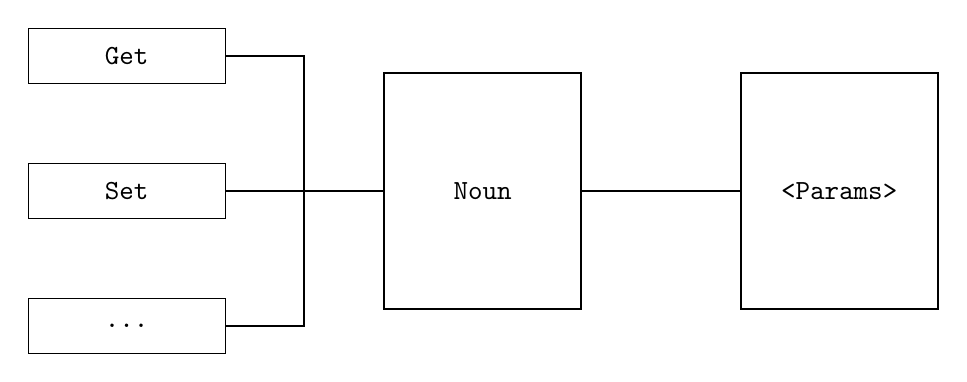
\begin{tikzpicture}[
    node distance=1cm and 2cm, % Abstand zwischen den Knoten
    every node/.style={font=\sffamily}, % Schriftart der Knoten
    noun/.style={draw, thick, align=center, minimum height=3cm, minimum width=2.5cm}, % Stil des Noun
    verb/.style={draw, align=center, minimum width=2.5cm, minimum height=0.7cm}, % Stil der Verbs
    param/.style={draw, thick, align=center, minimum height=3cm, minimum width=2.5cm} % Stil der Params-Box
]

% Noun-Knoten
\node[noun] (noun) {\texttt{Noun}};

% Param-Knoten (rechts von Item)
\node[param] (params) [right=of noun] {\texttt{<Params>}};

% Verb-Knoten
\node[verb] (get) [left=of noun.north west, yshift=0.2cm] {\texttt{Get}};
\node[verb] (set) [below=of get] {\texttt{Set}};
\node[verb] (new) [below=of set] {\texttt{...}};

% Verbindungslinien
\draw[thick] (get.east) -- ++(1cm,0) |- (noun.west);
\draw[thick] (set.east) -- ++(1cm,0) |- (noun.west);
\draw[thick] (new.east) -- ++(1cm,0) |- (noun.west);

% Verbindung zwischen Item und Params
\draw[thick] (noun.east) -- (params.west);

\end{tikzpicture}
\end{center}

\end{document}
